\documentclass{article}
\input{../../../../LaTex/preamble/preamble_article.tex}


\title{专题:动态分析+关联速度+拉密习题+重绳问题}
\author{教师: 马祥芸}


\begin{document}
\maketitle
\tableofcontents
\zihao{-4}
\newpage


\section{动态受力分析}
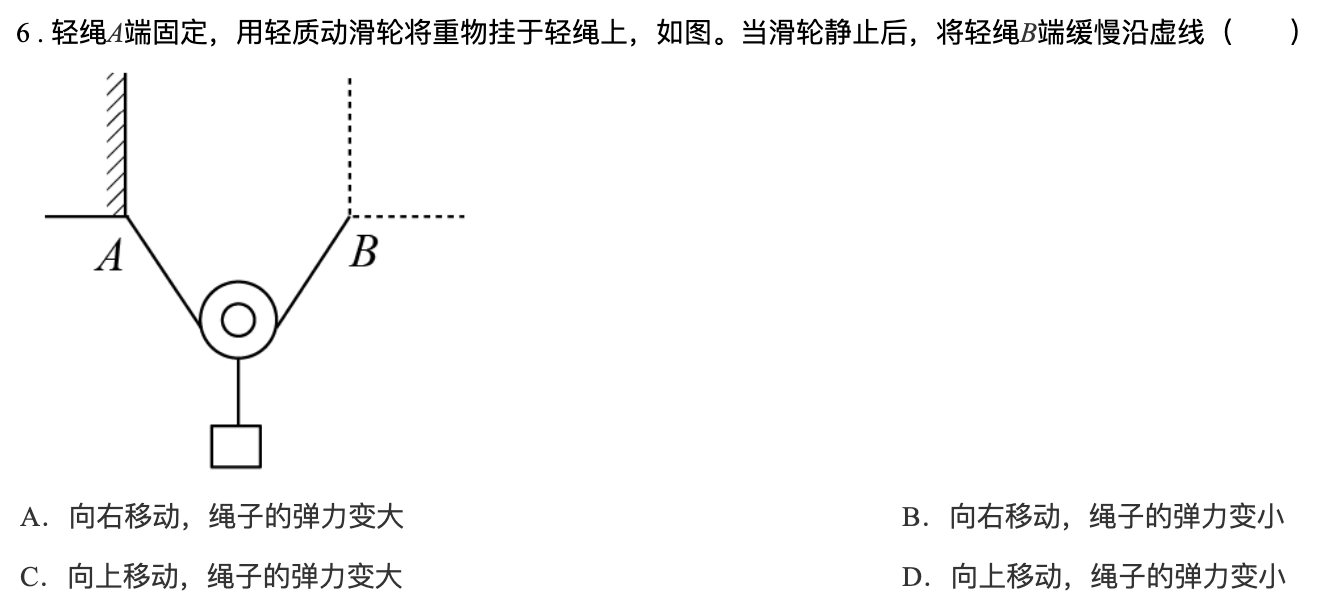
\includegraphics[width = 0.95\textwidth]{./pictures/1-1.png}

\vspace{5em}

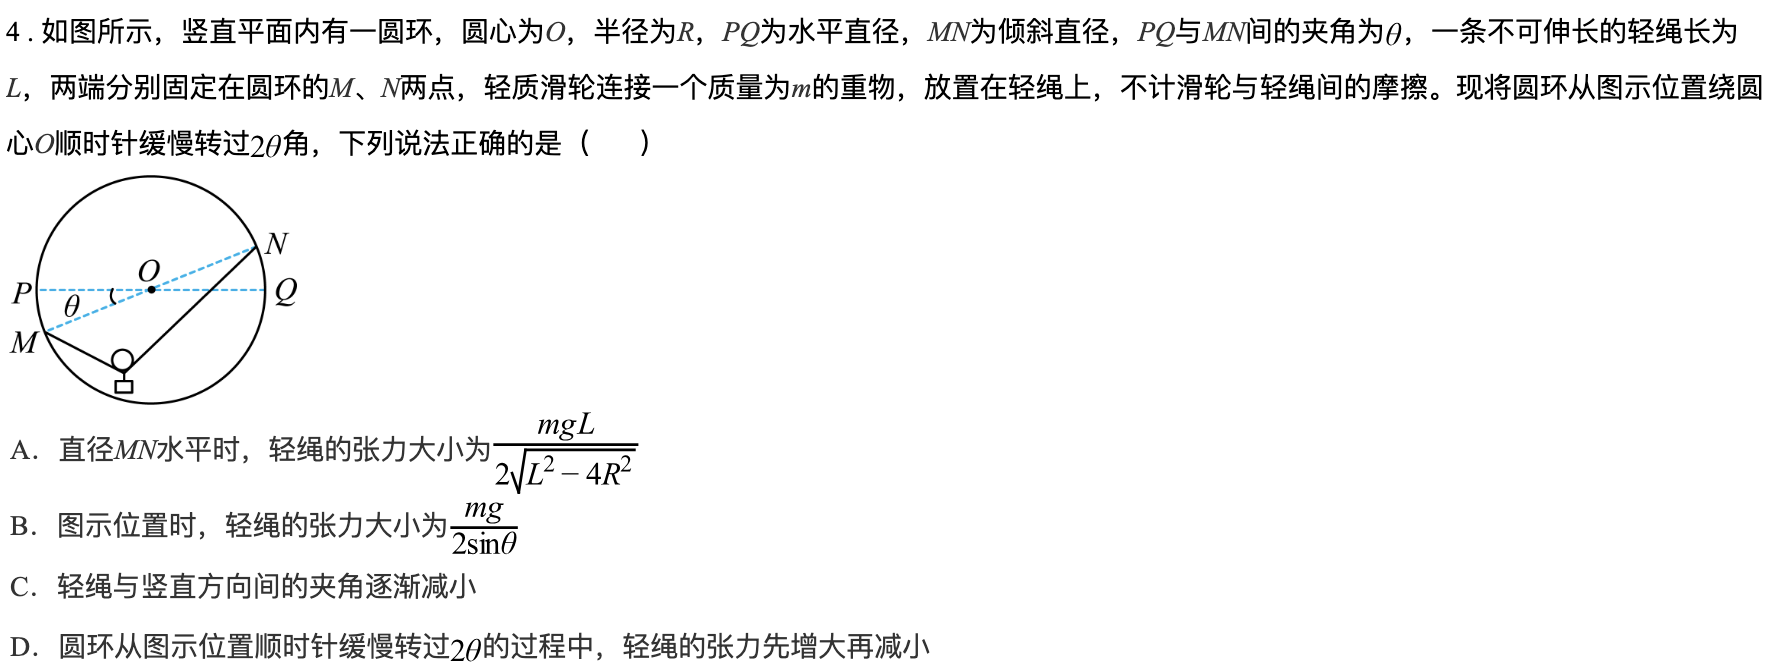
\includegraphics[width = 0.95\textwidth]{./pictures/1-2.png}

\vspace{5em}

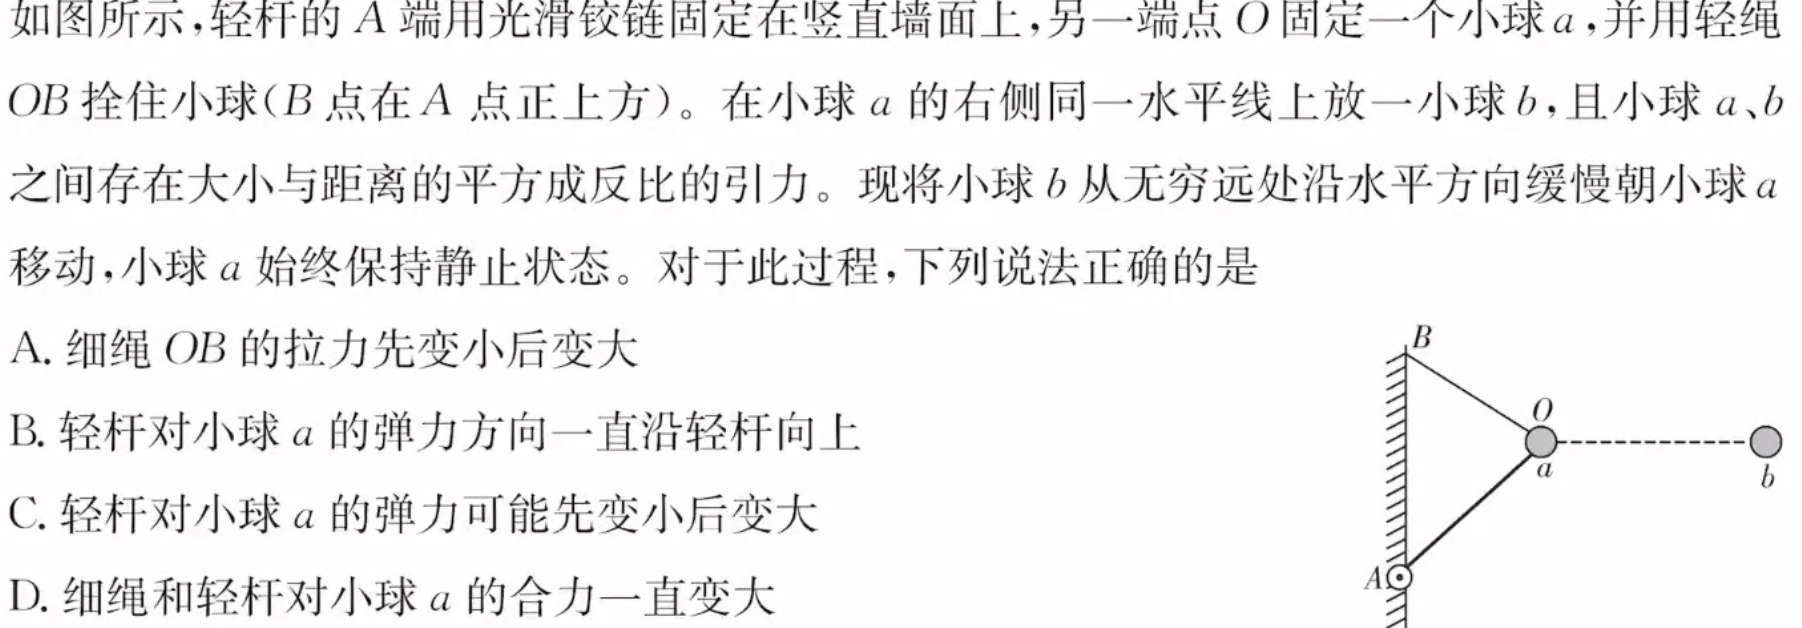
\includegraphics[width = 0.95\textwidth]{./pictures/1-3.png}

\vspace{5em}

\section{绳的关联速度}
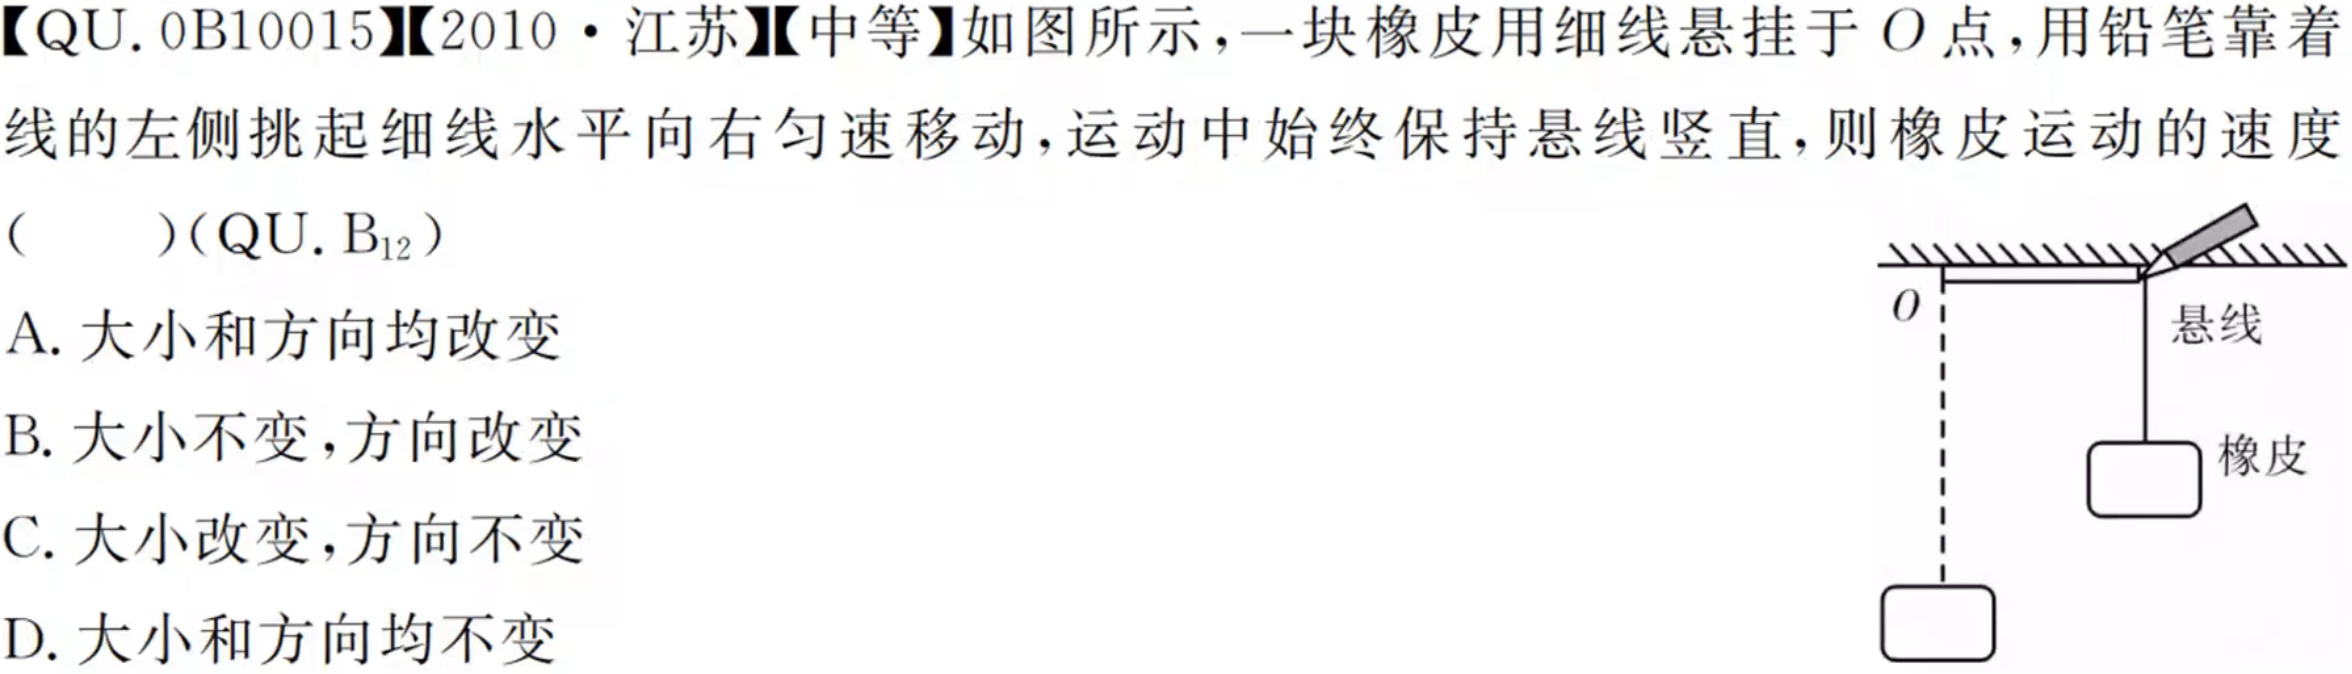
\includegraphics[width = 0.95\textwidth]{./pictures/2-1.png}

\vspace{10em}

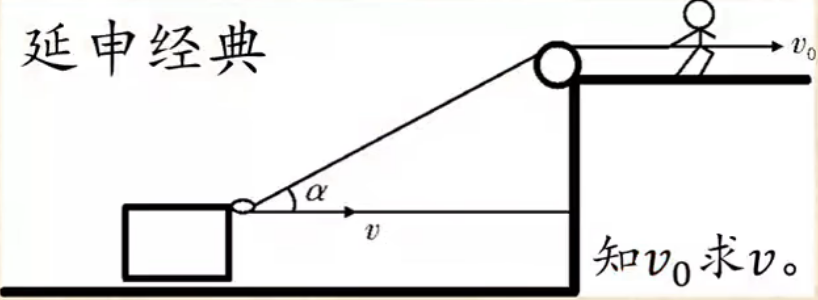
\includegraphics[width = 0.8\textwidth]{./pictures/2-2.png}

\vspace{5em}

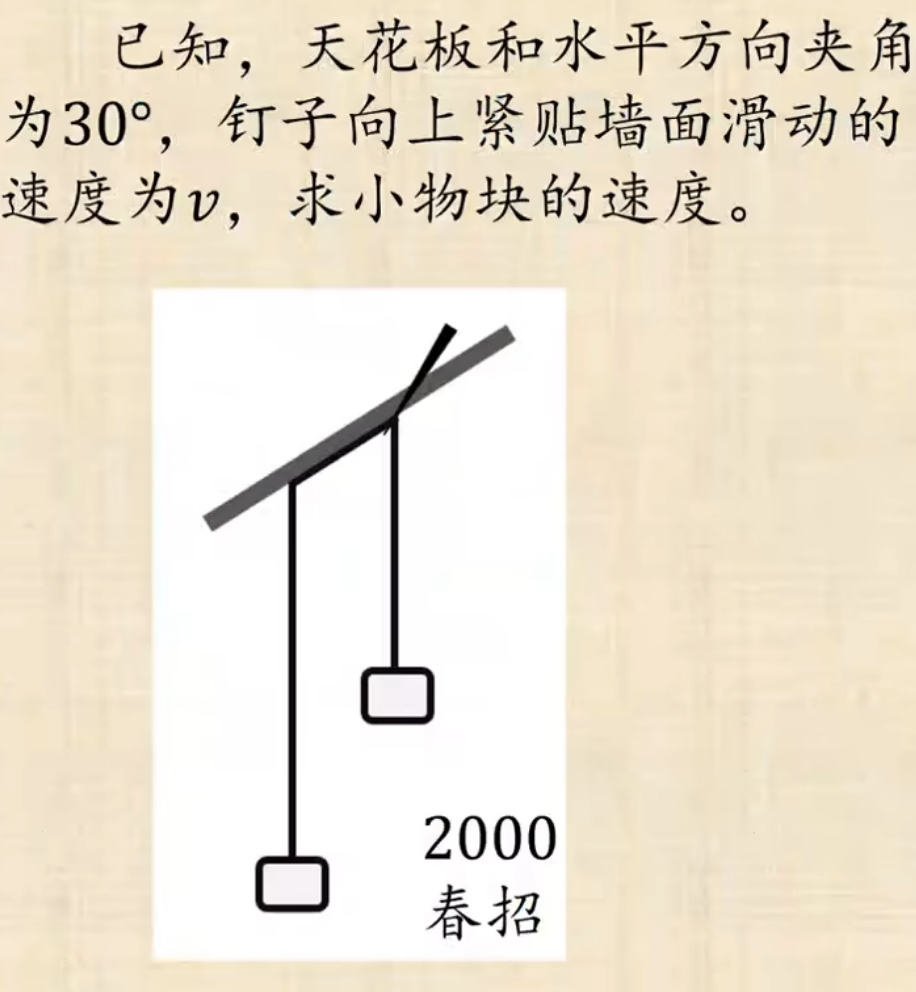
\includegraphics[width = 0.8\textwidth]{./pictures/2-3.png}

\vspace{5em}

\section{拉密习题}
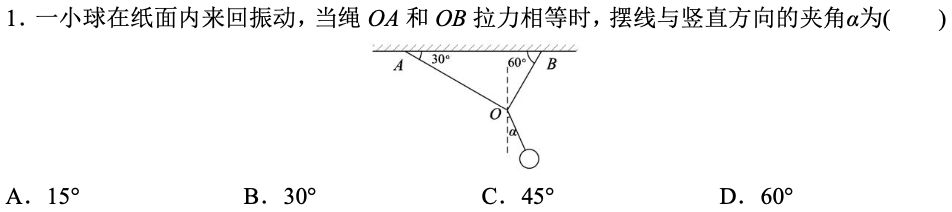
\includegraphics[width = 0.95\textwidth]{./pictures/3-1.png}

\vspace{5em}

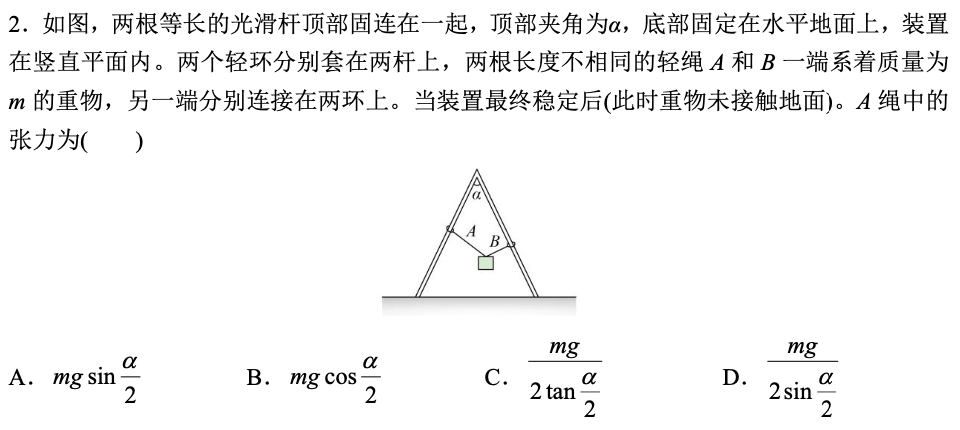
\includegraphics[width = 0.95\textwidth]{./pictures/3-2.png}

\vspace{5em}

\section{重绳问题}
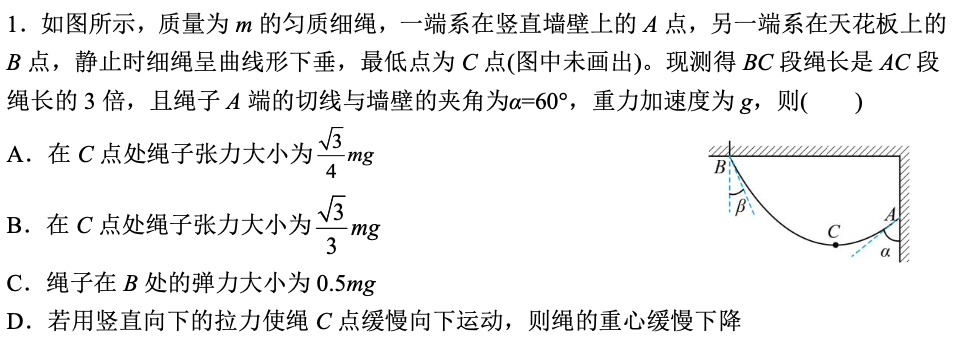
\includegraphics[width = 0.95\textwidth]{./pictures/4-1.png}

\vspace{5em}

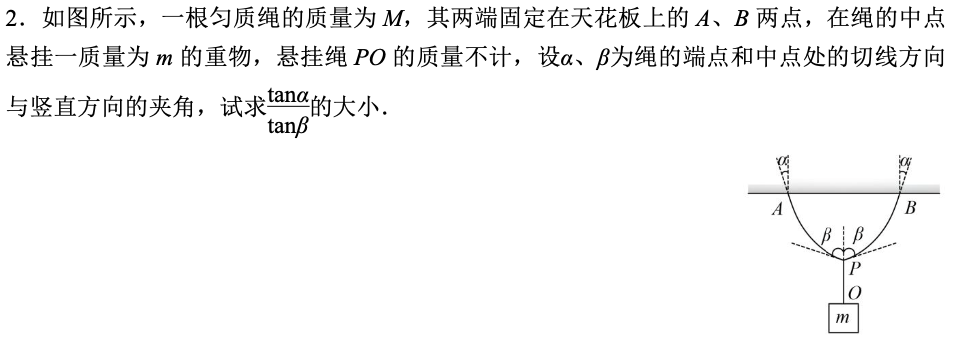
\includegraphics[width = 0.95\textwidth]{./pictures/4-2.png}

\vspace{5em}

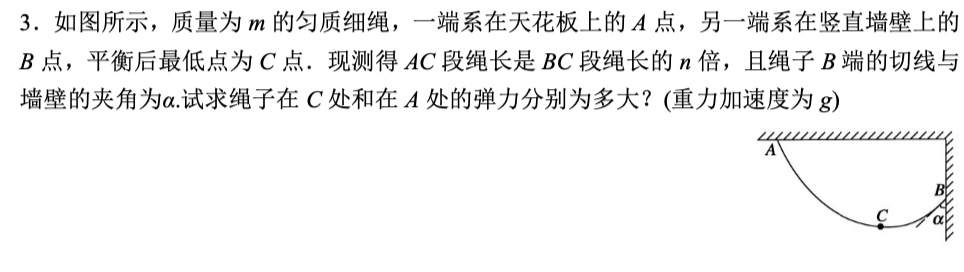
\includegraphics[width = 0.95\textwidth]{./pictures/4-3.png}

\newpage

\section{参考答案}

\begin{minipage}{0.5\textwidth}
    \begin{itemize}
        \item 动态受力分析
              \begin{enumerate}
                  \item A
                  \item AD
                  \item CD
              \end{enumerate}
        \item 绳的关联速度
              \begin{enumerate}
                  \item D
                  \item $v = \frac{v_{0}}{1+\cos{\alpha}}$
                  \item $\sqrt{3}v$
              \end{enumerate}

        \item 拉密习题
              \begin{enumerate}
                  \item $A \quad \sin{(150^{\circ} - \alpha)} = \sin{(120^{\circ} + \alpha)}$
                  \item $D \quad \text{做结点水平线,再由平行关系和等腰关系得到}$
                  
                  $\frac{T_{A}}{\sin{(\frac{\pi}{2} + \frac{\alpha}{2})}} = \frac{mg}{\sin{\alpha}}$
              \end{enumerate}

        \item 重绳
              \begin{enumerate}
                  \item A
                  \item $\frac{m}{m+M}$
                  \item $F_{B} \cos{\alpha} = \frac{1}{1+n} \, mg \quad F_{B} \sin{\alpha} = T$ 
                  \item[]$T = \frac{mg}{n+1} \, \tan{\alpha}    \quad T_{A} \sin{\beta} = \frac{n}{n+1} \, mg$
                  \item[]$T_{A} \cos{\beta} = T^{'}_{C} \quad T_{C} = T^{'}_{C}$
                  \item[]$\lra T_{A} = \frac{mg}{n+1} \sqrt{n^{2} + \tan^{2}{\alpha}}$
              \end{enumerate}
    \end{itemize}
\end{minipage}















\end{document}